\documentclass[10pt, compress,xcolor={svgnames,dvipsnames,x11names}]{beamer}
%\documentclass[10pt, compress,xcolor={svgnames,dvipsnames,x11names},trans]{beamer}
\usepackage[utf8]{inputenc}
\usepackage[T1]{fontenc}
\usetheme{metropolis}

% Pasta das imagens
\graphicspath{{../images/presentation}}
% Ajustando o tamanho da fonte nas legendas
\setbeamerfont{caption}{size=\tiny}
\setbeamerfont{caption name}{series=\bfseries}

% Introdução da logo da EESC no título
\titlegraphic{\vspace{5cm}\hspace*{8cm}\includegraphics[width = 2.5cm]{../images/presentation/logoEESC.pdf}}
\title{Design and Simulation of Microgrid Coopertative Multi-Agent Pinning-Based Droop Control}

\subtitle{Masters Thesis qualification exam}

\date{May 02, 2019}
\author{Álvaro Augusto Volpato}
\institute{
Advisor Prof. Luís Fernando C. Alberto\\
São Carlos School of Engineering\\
University of São Paulo\\
Department of Electrical and Computer Engineering 
}


%-----------------------------------------------------------------------------------------------------------------------
% DOCUMENT START
%-----------------------------------------------------------------------------------------------------------------------
\begin{document}

\maketitle

%-----------------------------------------------------------------------------------------------------------------------
\section{Introduction}%{{{1
%-----------------------------------------------------------------------------------------------------------------------

\begin{frame}%{{{2
\frametitle{Centralized Generation}

	Due to the rapid industrialization of the 20th century and the development of coemmercially available electrical home appliances, Electric Power Systems worldwide were developed under a universal paradigm called Centralized Generation (CG). In this paradigm, large power plants are built close to the prime fuel source and electric energy is supplied to a wide geographical area through transmission lines. To distribute energy a sophisticated system of substation and transmission lines is used to monitor and distribute energy radially among consumers.
	
\end{frame}%}}}2

\begin{frame}%{{{2
\frametitle{CG characteristics}

\begin{enumerate}[<+->]
	\item \textbf{Bulk power demand}: the energy market has become an economy of scale due to the developments in turbine size increase, decreasing marginal production cost;
%
	\item \textbf{Maximum efficiency}: due to the inherent transmission loss, there is a perennial effort to develop new transmission and distribution technologies;
%
	\item \textbf{System stability and reliability}: as the system takes huge proportions, it can be asily instabilized and disturbed by events like short-circuits, faults and generator losses. Hence stabilizing techniques are needed to continuously adjust the system to an operational safe state, eventually restoring it into operation after a breakdown.
\end{enumerate}
	
\end{frame}%}}}2

\begin{frame}%{{{2
\frametitle{CG downsides}

\begin{enumerate}[<+->]
	\item \textbf{Transmission cost}: by the 1970s the economies of scale started failing. Due to the transmission losses, the transmission system became more expensive than power plants themselves, due to maintenance and investment costs.  Because of this, utilities were unable to provide competitive prices;
%
	\item \textbf{Unreliability}: the transmission system spans wide geographical areas, meaning it is prone to disturbance events. This makes energy unreliable, specially in remote areas where maintenance is difficult;
%
	\item \textbf{Environmental concertns}: CG technologies are generally have deep environmental effects. Around 60\% of U.S. total electric energy production and 70\% of the chinese production is based on fossile fuels (U.S. E.I.A (2018); C.E.C (2018)). 
\end{enumerate}
	
\end{frame}%}}}2

\begin{frame}%{{{2
\frametitle{Environmental concerns}

	The environmental concerns with energy generation were the main driving factors behind the development of Renewable Power Generation Technologies (RPGTs).

	After a historical worldwide effort with the Kyoto Protocol and its subsequent accord, heavy investiments were made in RPGTs to generate cleaner energy.

	Nowadays these technologies are able to generate enough energy to power most small to medium-scale demands. Nevertheless, these technologies are not suitable to be employed in the Centralized Distribution paradigm.
	
\end{frame}%}}}2

\begin{frame}%{{{2
\frametitle{The Chinese Example}

	China is the worlds leading producer of solar panels, solar energy and wind energy, and has the largest installed photovoltaic and wind capacity worldeide, making yearly massive investments in the energy industry.

	Nevertheless, the heavy reliance of the chinese grid on fossile fuels, space limitation and the bureaucracy are major obstacles to implementation of reneweable power plants, small or large ones.

	Also the grid transmission capability is not able to keep up with the growth in installed capability, as only 84\% of installed wind and photovoltaic capacity is connected to the grid.
	
\end{frame}%}}}2

\begin{frame}%{{{2
\frametitle{Why RPGTs are mostly used im Microgrids}

\begin{enumerate}[<+->]
	\item \textbf{Affordable implementation}: large-scale plants need enourmous investments, while small distributed grids can be implemented by the users, developing an energy market and commerce;
%
	\item \textbf{Widespread use}: PV and wind generation have been amployed in small systems for decades now, meaning that there already are wwll-understood control and supervision techniques available;
%
	\item \textbf{High efficiency and reliability}: due to the lack of transmission lines and the advent of power electronics, small-scale systems have reached up to 95\% efficiency values. These systems are also reliable since they are equipped with security measures.
\end{enumerate}
	
\end{frame}%}}}2

%-----------------------------------------------------------------------------------------------------------------------
\section{The control problem}%{{{1
%-----------------------------------------------------------------------------------------------------------------------

\begin{frame}%{{{2
\frametitle{The Stability Problem}

	``Stability'' in EPSs refers to the capability of restoring a safe operating state after disturbance. In short terms, this means keeping all agents operating under the same frequency and voltage levels.

	Hence an EPS is considered ``safe'' or ``stable'' if able to withstand a list of plausible contingencies and wors-case scenarios listed by the designer or operator.

	In this sense, stability studies generally follow a well-defined procedure: applying the listed contingencies to an algebraic-differential model and simulating the post-disturbance system through numeric solvers. If no operational or safety limits are exceeded the system is considered safe and the control techniques employed are deemed successful.
	
\end{frame}%}}}2

\begin{frame}%{{{2
\frametitle{Stability Problem Fields}

	Generally the main reason for loss of synchronism and or voltage collapse in EPSs is the unability to respond to active or reactive power demands. Because of this, the Stability Problem is usually broken in three areas:

\begin{itemize}
	\item \textbf{Voltage and frequency stability}: maintaining acceptable voltage and frequency levels. The unability to do so may cause electromechanical damage to consumers and generators, as well as malfunctioning of devices. Whilst voltage stability is generally related to reactive power supply, frequency stability is associated with active power flows;
%
	\item \textbf{Angle stability}: based on the nonlinear relation between power flows and voltage angles. In Synchronous Machines this is primarily due to the angular position of the rotors.
\end{itemize}
	
\end{frame}%}}}2

\begin{frame}%{{{2
\frametitle{Overgeneration}

	RPGTs are generally intermittent and variable, causing conventional generators to compensate for fluctuations --- causing voltage and frequency oscillations. In this regard, the CAISO report of 2013 shows the Duck Chart, which points two major problems:

\begin{enumerate}
	\item \textbf{Curtailment}: the minimal ``must-run'' power output of conventional facilities lioke hydro and thermal is not accomodated in the demand due to the over-penetration of PV in the system;
%
	\item \textbf{Demand ramp}: between 5 and 7pm, PV production falls while power demand rises in a short timespan, causing the conventional grid to be fastly accelerate, incurring damage in its generators.
\end{enumerate}

\end{frame}%}}}2

\begin{frame}%{{{2
\frametitle{The Duck Chart}

\begin{figure}[htb]
	\begin{center}
		\includegraphics[width = .8\textwidth]{../images/presentation/duck.png}
		\caption{Duck Chart showing the curtailment and demand ramp issues.}
		\label{fig:duck}
	\end{center}
\end{figure}

\end{frame}%}}}2

\begin{frame}%{{{2
\frametitle{Proper Load Sharing (PLS)}

	All generators have power ratings that must be respected to ensure proper operation. Big generators and small generators should contribute to the grid in the capacity of their ratings. Mathematically, this means every generator must output power proportionately to their rated limits.

	The main issue with PLS is that by dynamic properties, smaller generators tend to take on more load responsibility as their rotor acceleration is facilitated by lower inertia.

	PLS has also seen a concept revision as many RPGTs are non-dispatchable power resources that follow a Maximum Power Tracking --- which is fundamentally the reason for the curtailment problem shown in the Duck Curve.

\end{frame}%}}}2


%-----------------------------------------------------------------------------------------------------------------------
\section{O sistema OMIB}%{{{1
%-----------------------------------------------------------------------------------------------------------------------
\begin{frame}%{{{2
\frametitle{Caracterização}
\scriptsize

	O sistema é baseado naquele utilizado por Concordia e DeMello em \cite{concordia}. Os parâmetros da máquina e do sistema estão especificados na tabela 1, página 26.

	\begin{center}
		\begin{figure}
			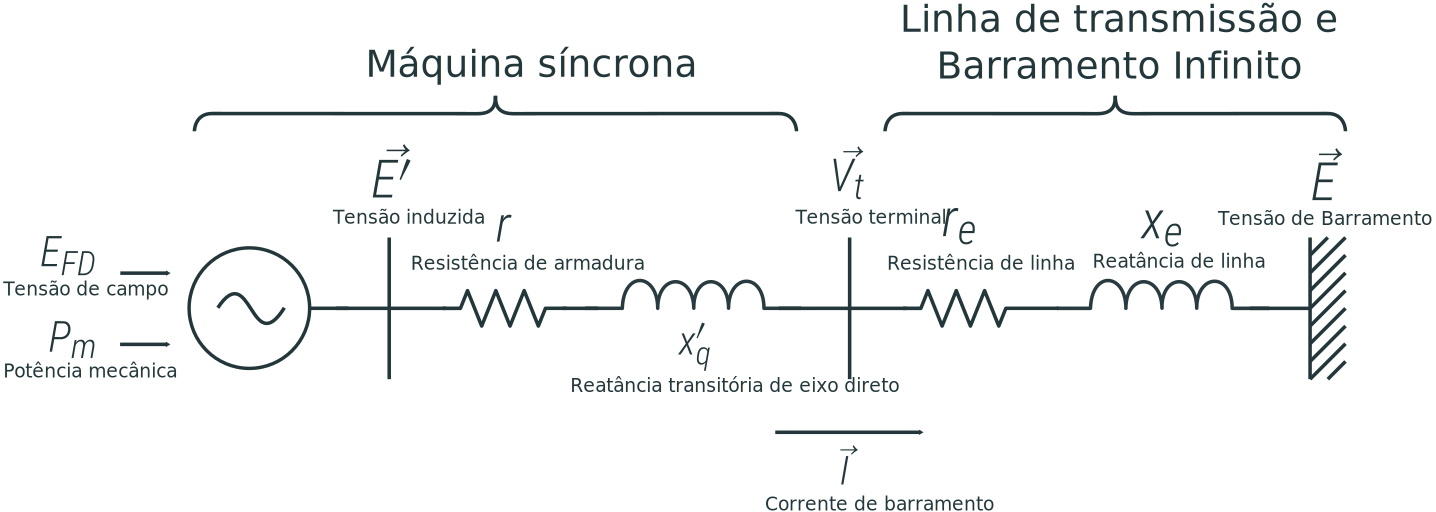
\includegraphics[width = 1\textwidth]{../images/presentation/gerador.pdf}
			\caption{Esquemático do sistema OMIB}
			\label{fig::figuraOMIB}
		\end{figure}
	\end{center}


\normalsize
\end{frame}%}}}2

%-----------------------------------------------------------------------------------------------------------------------
\begin{frame}%{{{2
\frametitle{Modelo de perturbação}
\scriptsize

	O modelo de perturbação adotado será um degrau na potência mecânica do sistema. O degrau tem amplitude $\Delta P$, ocorre num dado instante de tempo $t_P$, e ocorre em relação à potência mecânica em equilíbrio $P_{m0}$.

\begin{gather}
P_m\left(t,t_P\right) = P_{m0} + u\left(t - t_P\right)\Delta P
\end{gather}

	$\Delta P$ é da ordem de porcento de p.u., geralmente de $1\%$ a $10\%$.

\normalsize
\end{frame}%}}}2

%-----------------------------------------------------------------------------------------------------------------------
\section{Hipóteses simplificadoras}%{{{1
%-----------------------------------------------------------------------------------------------------------------------
\begin{frame}%{{{2
\frametitle{Hipótese 1: modelo de um eixo}
\scriptsize

	As suposições e os resultados se debruçam sobre algumas suposições que advêm do \alert{modelo de um eixo} utilizado para o gerador síncrono e das características da máquina:

	\begin{itemize}
		\item A componente de eixo direto da tensão interna da máquina $E'_d$ é desprezível em qualquer instante de tempo;
		\item O regime subtransitório da máquina pode ser desprezado por sua brevidade; 
	\end{itemize}

\normalsize
\end{frame}%}}}2

%-----------------------------------------------------------------------------------------------------------------------
\begin{frame}%{{{2
\frametitle{Hipótese 2: máquina com rotor de pólos lisos}
\scriptsize

	A máquina em estudo possui rotor de pólos lisos. Advém que as impedâncias equivalentes transitórias de eixo direto e em quadratura ($x'_d$ e $x'_q$, respectivamente) são próximas devido à relutância simétrica do rotor.

	Apenas através desta simplificação é possível representar o sistema como na figura \ref{fig::figuraOMIB}. Outrossim, se a máquina não for de pólos lisos então ela não pode ser representada através de um gerador ideal seguido de uma resistência equivalente de armadura $r$ e uma impedância $x'_q \approx x'_d$.

\normalsize
\end{frame}%}}}2

%-----------------------------------------------------------------------------------------------------------------------
\begin{frame}%{{{2
\frametitle{Hipótese 3: O barramento infinito}
\scriptsize

	O barramento infinito representa um sistema muito maior que a máquina, ordens de magnitude mais influente; assim, a contribuição de uma máquina em especial é negligenciável: a tensão, fase e corrente da barra são constantes independentemente de carga . Dessa forma, o que chamou-se de ``impedância equivalente de linha'' e a própria tensão do barramento são, na verdade, parâmetros equivalentes de Thévenin do sistema ao qual a máquina é acoplada, e cuja inércia é tão maior que a da máquina a ponto de poder ser considerada infinita.

	A influência irrsória da máquina ao barramento infinito é equiparável à influência do pêndulo de massa negligenciável perante àquela da Terra.

\normalsize
\end{frame}%}}}2

%-----------------------------------------------------------------------------------------------------------------------
\begin{frame}%{{{2
\frametitle{Sistema sem controladores}
\scriptsize

	O sistema OMIB, em malha aberta, é regida segundo o sistema algébrico-diferencial a seguir, deduzido em \cite{livroDoLfComORodrigoEOBretas}:

\begin{columns}[T]
\begin{column}{0.5\textwidth}
\begin{align} \label{sis::sistemaDiferencialMalhaAberta}
\left\{ \begin{array}{l}
\dot{x_1} = \dfrac{x_4 - x_1 + \left(\strut x_d - x'_d \right)I_d}{T'_{do}} \\[4mm]
%
\dot{x_2} = \dfrac{P_m - x_1 I_q + \left(\strut x'_d - x'_q \right)\ I_d I_q}{2H}\\[4mm]
%
\dot{x_3} = x_2\\[4mm]
%
\dot{x_4} = 0\\[4mm]
%
I_q = \dfrac{x_1\cos\left(\phi\right) - E\cos(x_3 + \phi) }{X} \\[2mm]
%
I_d = \dfrac{E\sin(x_3 + \phi) - x_1\sin(\phi) }{X}
\end{array}\right.
\end{align}
\end{column}

\begin{column}{0.5\textwidth}
\vspace{1cm}
Sendo:

\begin{itemize}
	\item $E'_q = x_1$  a tensão interna induzida da máquina; 
	\item $\omega = x_2$ a velocidade angular do rotor com relação ao eixo QD;	
	\item $\delta = x_3$ o ângulo do rotor com relação do eixo QD;
	\item $E_{FD} = x_4$ a tensão no enrolamento de campo, que no sistema em malha aberta é constante e igual ao valor inicial;
		\item $\vec{X} = \left(\strut r + r_e \right) + j\left(x'_q + x_e\right) = Xe^{j\phi}$ a impedância total equivalente;
\end{itemize}
\end{column}
\end{columns}

\normalsize
\end{frame}%}}}2

%-----------------------------------------------------------------------------------------------------------------------
\section{Cálculo do balanço de potência}%{{{1
%-----------------------------------------------------------------------------------------------------------------------
\begin{frame}%{{{2
\frametitle{Cálculo da corrente de barramento}
\scriptsize

	Inicialmente, a máquina se encontra num estado de operação, fornecendo ao sistema uma potência elétrica aparente $\vec{S} = P + jQ = 1 + j0.5 \ VA$. Nesse momento, a potência mecânica fornecida à máquina é $P_m = 1\ p.u.$. As equações de fluxo de potência resultam:

\begin{equation}
\vec{S} = \left[\left(\strut r + r_e\right) + j\left(\strut x'_d + x_e\right)\right]\times | \vec{I} |^2 + E\times \vec{I^{*}} \Leftrightarrow
%
\left\{ \begin{array}{ll}
\left(Re\right): & P = r_t(I_r^2 + I_i^2) + E\ I_r \label{eq:inicial1}\\[2mm]
%
\left(Im\right): & Q = x_t(I_r^2 + I_i^2) - E\ I_i 
\end{array} \right.
\end{equation}

\begin{gather}
\left\{ \begin{array}{l}
0 = I_r^2 \left[E^2\left(\strut x_t^2 + r_t^2\right)\right] + I_r \left[ r_tE^3 + 2x_tE\left(\strut Qr_t - Px_t \right)\right] + \left[\left(\strut Qr_t - Px_t \right) ^2 -r_tPE^2\right]\\[2mm]
%
I_i = \dfrac{Px_t - Qr_t}{Er_t} - \dfrac{x_t}{r_t}I_r
\end{array}  \right.\label{sis::sistemaPontoDeOperacaoCorrentes} 
\end{gather}

	Onde $\vec{I} = \left( I_r\ ,\ I_I\right)$ é a corrente de barramento, decomposta nas suas componentes real e imaginária. A referência de fase zero do eixo é a tensão de barramento infinito. 

\normalsize
\end{frame}%}}}2

%-----------------------------------------------------------------------------------------------------------------------
\begin{frame}%{{{2
\frametitle{Calculo das tensões e versores do rotor}
\scriptsize

	De posse das equações que definem a corrente de barramento, podem-se calcular as tensões das barras:

\begin{align}
\begin{array}{cr}
	\vec{V_t} = E + \left(\strut r_e + jx_e\right)\vec{I} & \text{(\ref{sis::tensoesEquilibrio}.a)} \\[2mm]
	\vec{E'} = \vec{V_t} + \left(\strut r + jx'_q\right)\vec{I} & \text{(\ref{sis::tensoesEquilibrio}.b)}
\end{array}\label{sis::tensoesEquilibrio}
\end{align}

	Falta agora transformar estas grandezas para o eixo QD. Para descobrir a posição deste eixo em relação ao imaginário, utiliza-se do fato que, em se tratando de um modelo de um eixo, então $\vec{E'}$ está em fase com o eixo Q, de forma que

\begin{equation}
	\vec{Q} = \frac{\vec{E'}}{|\vec{E'}|} \Leftrightarrow 	\delta = arg\left(\strut \vec{Q}\right) = arg\left(\strut \vec{E'}\right) 
\end{equation}

seja o versor unitário do eixo Q. Girando $\vec{Q}$ de noventa graus, obtém-se o versor do eixo direto $\vec{D}$, quer dizer: se $\vec{Q} = (a,b) \Leftrightarrow \vec{D} = (-b,a)$.

\normalsize
\end{frame}%}}}2

%-----------------------------------------------------------------------------------------------------------------------
\begin{frame}%{{{2
\frametitle{Calculo das tensões e correntes no eixo QD}
\scriptsize

	Calculam-se assim as mesmas grandezas no eixo QD do rotor, através de

\begin{align}
	E'_q &= \vec{E'} \cdot \vec{Q} = \phantom{-}\text{Re}\left(\vec{E'}\right)\cos\left(\delta\right) + \text{Im}\left(\vec{E'}\right)\sin\left(\delta\right) \label{eq::QDinicio}\\
	E'_d &= \vec{E'} \cdot \vec{D} = -\text{Re}\left(\vec{E'}\right)\sin\left(\delta\right) + \text{Im}\left(\vec{E'}\right)\cos\left(\delta\right)\alert{=0}  \\[5mm]
%
	V_q &= \vec{V_t} \cdot \vec{Q} = \phantom{-}\text{Re}\left(\vec{V}\right)\cos\left(\delta\right) + \text{Im}\left(\vec{V}\right)\sin\left(\delta\right) \\
	V_d &= \vec{V_t} \cdot \vec{D} = -\text{Re}\left(\vec{V}\right)\sin\left(\delta\right) + \text{Im}\left(\vec{V}\right)\cos\left(\delta\right)  \\[5mm]
%
	I_q &= \vec{I} \cdot \vec{Q} = \phantom{-}\text{Re}\left(\vec{I}\hspace{1mm}\right)\cos\left(\delta\right) + \text{Im}\left(\vec{I}\hspace{1mm}\right)\sin\left(\delta\right)  \\
	I_d &= \vec{I} \cdot \vec{D} = - \text{Re}\left(\vec{I}\hspace{1mm}\right)\cos\left(\delta\right) + \text{Im}\left(\vec{I}\hspace{1mm}\right)\sin\left(\delta\right) \label{eq::QDfinal}
\end{align}
\normalsize
\end{frame}%}}}2

%-----------------------------------------------------------------------------------------------------------------------
\begin{frame}%{{{2
\frametitle{Aplicando as equações de equilíbrio}
\scriptsize

	De posse das equações de fluxo de potência e do sistema diferencial da máquina, pode-se calcular os parâmetros em equilíbrio aplicando $\dot{\mathbf{x}} = 0$, daonde

\begin{gather}
\left\{ \begin{array}{l}
\dot{x_1} = \dfrac{x_4 - x_1 + \left(\strut x_d - x'_d \right)I_d}{T'_{do}} \\[4mm]
%
\dot{x_2} = \dfrac{P_m - x_1 I_q + \left(\strut x'_d - x'_q \right)\ I_d I_q}{2H}\\[4mm]
%
\dot{x_3} = x_2\\[4mm]
%
\dot{x_4} = 0\\[4mm]
%
I_q = \dfrac{x_1\cos\left(\phi\right) - E\cos(x_3 + \phi) }{X} \\[2mm]
%
I_d = \dfrac{E\sin(x_3 + \phi) - x_1\sin(\phi) }{X}
\end{array}\right. \Leftrightarrow 
\left\{\begin{array}{cl}
	E_{FD0} &= E'_{q0} - \left(\strut x_d - x'_d \right)I_{d0} \\[2mm]
	%
	P_{m0} &= E'_{q0}I_{d0} - \left(x'_d - x'_q \right)I_{d0}I_{q0} \\[2mm]
	%
	\omega_0 &= 0 \\[3mm]
	%
	\alert{ I_{q0} } &= \alert{ \dfrac{E'_{q0}\cos\left(\phi\right) - E\cos(\delta_0 + \phi) }{X} }\\[3mm]
	%
	\alert{I_{d0}} &= \alert{\dfrac{E\sin(\delta_0 + \phi) - E'_{q0}\sin(\phi) }{X}}
\end{array}\right.\label{sis::equilibrio}
\end{gather}

	As últimas duas equações estão destacadas pois são redundantes, uma vez que a corrente de barramento já foi calculada através do balanço de potência; foram adicionadas por bem da completude e integração do modelo com as equações daquele balanço de potência. Quer dizer: os resultados têm que coincidir.

\normalsize
\end{frame}%}}}2

%-----------------------------------------------------------------------------------------------------------------------
\begin{frame}%{{{2
\frametitle{Algoritmo para cálculo do ponto de equilíbrio}
\scriptsize

\begin{enumerate}
	\item De posse da potência aparente $\vec{S}$ que a máquina entrega ao sistema, calcular a corrente de barramento através de \ref{sis::sistemaPontoDeOperacaoCorrentes};
	%
	\item Calcular as tensões terminais $\vec{V_t}$ e $\vec{E'}$ através de (\ref{sis::tensoesEquilibrio}.a) e (\ref{sis::tensoesEquilibrio}.b);
	%
	\item Obter o versor do eixo de quadratura $\vec{Q}$ e seu argumento $\delta$ para então rotacionar as tensões e correntes calculadas anteriormente e obtê-las no eixo QD;
	%
	\item Finalmente, obter a tensão de campo, potência mecânica desenvolvida e frequência do rotor no equilíbrio através do sistema \ref{sis::equilibrio}.
\end{enumerate}

\normalsize
\end{frame}%}}}2

%-----------------------------------------------------------------------------------------------------------------------
\begin{frame}%{{{2
\frametitle{Diagrama de condições iniciais do sistema em estudo}
\scriptsize

\begin{figure}[htb]
	\begin{center}
	    \includegraphics[width = 0.9\columnwidth]{../images/presentation/diagramaCondicoesIniciais.pdf}
	\end{center}
	\caption{\label{fig::diagramaCondicoesIniciais} Diagrama das condições iniciais para a máquina em estudo, com $\vec{S} = 1 + j0.5$.}
\end{figure}

\normalsize
\end{frame}%}}}2

%-----------------------------------------------------------------------------------------------------------------------
\section{Região de Factibilidade} %{{{1
%-----------------------------------------------------------------------------------------------------------------------
\begin{frame}%{{{2
\frametitle{Região de Factibilidade}
\scriptsize

	As equações de fluxo de potência (sistema \ref{sis::sistemaPontoDeOperacaoCorrentes}) nem sempre têm solução. A existência de solução está atrelada ao determinante

\begin{gather}
\Delta = \left[ r_tE^3 + 2x_tE\left(\strut Qr_t - Px_t \right)\right]^2 - 4E^2\left(\strut x_t^2 + r_t^2\right)\left[\left(\strut Qr_t - Px_t \right) ^2 -r_tPE^2\right] \geq 0 \nonumber
\end{gather}

	Assim, se faz necessária uma análise da existência de solução frente à escolha do ponto de operação $\vec{S} = P + jQ$. Pode-se mostrar que ele tem a forma

\begin{gather}
\dfrac{\Delta}{E^2r_t^4} = \left(\strut - 4z^2 \right)P^2 + \left(\strut 8z \right) PQ + \left(\strut -4 \right) Q^2 + \left[ - \left( 1+2z^2\right)\dfrac{E^2}{r_t} \right] P + \left(\strut 2z\dfrac{E^2}{r_t} \right) Q + \dfrac{E^4}{r_t^2} \geq 0 \label{eq::regiaoDeFactibilidadePQ}
\end{gather}

	, com $z = \dfrac{x_t}{r_t}$. Define-se então a \alert{Região de Factibilidade} como o lugar geométrico dos pontos $\left(\strut P\ ,\ Q\right)$ que satisfazem à inequalidade.

\normalsize
\end{frame}%}}}2

%-----------------------------------------------------------------------------------------------------------------------
\begin{frame}%{{{2
\frametitle{Forma da Região de Factibilidade}
\scriptsize

	Fazendo uma rotação de eixos para eliminar o termo retângulo em \ref{eq::regiaoDeFactibilidadePQ}:

\begin{equation}
\tan(\theta) = z
\end{equation}

 	origina-se um novo eixo $xy$ no qual a equação \ref{eq::regiaoDeFactibilidadePQ} tem a forma

\begin{align}
	\left(R_F\right):\ -\dfrac{r_t\left(\strut 1 + z^2\right)}{E^2} y^2 - \dfrac{1 + 4z^2}{\sqrt{1 + z^2}}x + \dfrac{z\left(\strut 1 - 2z^2 \right)}{\sqrt{1 + z^2}}y + \left(r_tE\right)^2 \geq 0 \label{eq::regiaoDeAlberto}
\end{align}

	Que sugere a equação de uma parábola de eixo horizontal e concavidade para a esquerda, pois o termo de $y^2$ é negativo sempre, bem como o termo de $x$.

\normalsize
\end{frame}%}}}2

%-----------------------------------------------------------------------------------------------------------------------
\begin{frame}%{{{2
\frametitle{Estudo da rotação dos eixos}
\scriptsize

	Nota-se que o ângulo $\theta$ é muito próximo de $\dfrac{\pi}{2}$ porque

\begin{equation}
\tan(\theta) = z = \dfrac{x_t}{r_t}
\end{equation}

	Como $r_t$ e $x_t$ são as componentes da impedância da linha de transmissão, e sabendo-se que esta tem forte característica indutiva, então $r_t$ é pequeno se comparado a $z_t$; logo a razão é grande e portanto $\theta$ é próximo do um quarto de volta, e tende a este valor pela esquerda. Assim, pode-se aplicar a função inversa arco-tangente porque $\theta$ será sempre menor que a metade de $\pi$ e logo estará sempre no intervalo de domínio da função arco-tangente: 

\begin{equation}
	D\left[\strut \arctan(.) \right] = \left[\strut\ -\dfrac{\pi}{2},\ \dfrac{\pi}{2}\ \right]
\end{equation}

	Pode-se assim aproximar $\theta$ pela expansão em Série de Laurent de $\arctan(.)$ em $x = \infty$:

\begin{equation}
\theta = \arctan(z) \approx \dfrac{\pi}{2} - \dfrac{1}{z}
\end{equation}

\normalsize
\end{frame}%}}}2

%-----------------------------------------------------------------------------------------------------------------------
\begin{frame}%{{{2
\frametitle{ Redução da equação para a forma canônica}
\scriptsize

	Reduzindo a equação da Região de Factibilidade \ref{eq::regiaoDeAlberto} à forma canônica da parábola:

\begin{equation}
	\left(\strut R_F\right): \left(\strut y - y_0 \right)^2 - 2p\left(\strut x - x_0 \right) \geq 0
\end{equation}

	Onde $p$ é o parâmetro da parábola e $\left(\strut x_0,\ y_0 \right)$ é o seu vértice. Então tem-se

\begin{align}
	y_0 =& \dfrac{E^2}{2r_t}\dfrac{z\left(\strut 1 - 2z^2\right)}{\sqrt{\strut \left(\strut 1 + z^2\right)^3}} \\[3mm]
	%
	x_0 =& \dfrac{E^2}{r_t}\dfrac{\sqrt{\strut 1 + z^2}}{\strut 1 + 4z^2} \left[\strut r_t^3 + \dfrac{z^2}{4}\left(\dfrac{1 - 2z^2}{1 + z^2}\right)^2 \right] \\[3mm]
	%
	p =& -\dfrac{2E^2}{r_t}\dfrac{1 + 4z^2}{\sqrt{\strut \left(\strut 1 + z^2\right)^3}}
\end{align}

\normalsize
\end{frame}%}}}2

%-----------------------------------------------------------------------------------------------------------------------
\begin{frame}%{{{2
\frametitle{ Redução da equação para a forma canônica}
\scriptsize

	Depois de rotacionar os eixos de $-\theta$, têm-se o ponto $\left(\strut P_0,\ Q_0\right)$ no plano PQ:

\begin{align}
		P_0  &= \dfrac{E^2}{r_t}\left\{\strut  \dfrac{1}{\strut 1 + 4z^2} \left[\strut r_t^3 + \dfrac{z^2}{4}\left(\dfrac{1 - 2z^2}{1 + z^2}\right)^2 \right] + \dfrac{z^2}{2}\dfrac{\left(\strut 2z^2 - 1\right)}{\left(\strut 1 + z^2\right)^2} \right\} \\[5mm]
		%
		Q_0 &=  \dfrac{E^2}{r_t}\left\{\strut  \dfrac{z}{\strut 1 + 4z^2} \left[\strut r_t^3 + \dfrac{z^2}{4}\left(\dfrac{1 - 2z^2}{1 + z^2}\right)^2 \right] - \dfrac{z}{2}\dfrac{\left(\strut 2z^2 - 1\right)}{\left(\strut 1 + z^2\right)^2} \right\}
\end{align}

	O valor $P_0$ corresponde aproximadamente à mínima potência ativa que a máquina pode fornecer ao sistema; $Q_0$ representa a potência reativa nesse ponto.
\normalsize
\end{frame}%}}}2

%-----------------------------------------------------------------------------------------------------------------------
\begin{frame}%{{{2
\frametitle{ Algoritmo para determinação da Região de Factibilidade }
\scriptsize

	Desenvolve-se assim o algoritmo com o fim de traçar a Região de Factibilidade do sistema:

\begin{enumerate}
	\item Calcula-se  $z = \dfrac{x_t}{r_t}$
%
	\item Calcula-se $\theta\left(z\right) = \arctan\left(\strut z\right) \approx \dfrac{\pi}{2} - \dfrac{1}{z}$:
%
	\item Traçar a Região de Factibilidade no eixo XY, segundo a equação

		\begin{align*}
			\left(R_F\right):\ -\dfrac{r_t\left(\strut 1 + z^2\right)}{E^2} y^2 - \dfrac{1 + 4z^2}{\sqrt{1 + z^2}}\ x + \dfrac{z\left(\strut 1 - 2z^2 \right)}{\sqrt{1 + z^2}}y + \left(r_tE\right)^2 \geq 0
		\end{align*}
%
	\item Rotacionar o eixo XY de $-\theta$, obtendo a região no eixo PQ;
%
	\item Calcular $P_0$ e $Q_0$.
\end{enumerate}

\normalsize
\end{frame}%}}}2

%-----------------------------------------------------------------------------------------------------------------------
\begin{frame}%{{{2
\frametitle{ Aplicação do algoritmo ao sistema em estudo }
\scriptsize

\begin{itemize}
	\item $z = \dfrac{x_t}{r_t} = \dfrac{0.24 + 0.1}{0 + 0.01} = 34 \Rightarrow \theta\left(34\right) = 1.276763445 = 0.406406427\pi $;
	%
	\item A equação da Região é

	\begin{align*}
		-289.25y^2 - 135.970613659x - 2310.001080567y + 0.01 &\geq 0 \Leftrightarrow \nonumber\\[2mm]
		%
		\Leftrightarrow - y^2 - 0.470079909x - 7.986174868y - 3.4572\times 10^{-5}  &\geq 0
	\end{align*}
%
	\item Esta equação no eixo XY é rotacionada ao eixo PQ, depictada na figura \ref{fig:regiaoDeFactibilidade}.
%
	\item O vértice é $\left(\strut P_0,Q_0\right) = \left(\strut -74.854208169278564, -850.5489706455613\right)$.  
\end{itemize}

\normalsize
\end{frame}%}}}2

%-----------------------------------------------------------------------------------------------------------------------
\begin{frame}%{{{2
\frametitle{ Aplicação do algoritmo ao sistema em estudo }
\scriptsize

\begin{figure}[htb]
	\begin{center}
	    \includegraphics[width = 0.8\columnwidth]{../images/presentation/regiaoDeFactibilidade.pdf}
	\end{center}
	\caption{\label{fig:regiaoDeFactibilidade} Região de Factibilidade do sistema em estudo, no equilíbrio $\vec{S} = 1 + j0.5$.}
\end{figure}

\normalsize
\end{frame}%}}}2

%-----------------------------------------------------------------------------------------------------------------------
\section{Comportamento dinâmico do sistema OMIB} %{{{1
%-----------------------------------------------------------------------------------------------------------------------
\begin{frame}%{{{2
\frametitle{Diagrama de blocos final do sistema}
\scriptsize

	Após ter o equilíbrio do sistema definido, bem como o sistema de DAEs definido, então estudam-se os controladores utilizados, AVR e PSS.

	O \textit{slide} a seguir mostra o sistema final pretendido. A seguir está o estudo do sistema controlado por AVR, e a ilustração temporal do seu comportamento dinâmico perante perturbação. Depois, estuda-se o sistema controlado por AVR e PSS (siustema ``AVR+PSS''), novamente plotando seus gráficos frente a perturbação.

\normalsize
\end{frame}%}}}2

%-----------------------------------------------------------------------------------------------------------------------
\begin{frame}%{{{2
\frametitle{Diagrama de blocos final do sistema}
\scriptsize

\begin{figure}[htb]
	\begin{center}
	    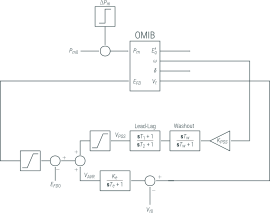
\includegraphics[width = 0.8\columnwidth]{../images/presentation/diagramaDeBlocos.pdf}
	\end{center}
	\caption{\label{fig::diagramaDeBlocos} Diagrama de blocos final do sistema em malha fechada, controlado por AVR e PSS.}
\end{figure}

\normalsize
\end{frame}%}}}2

%-----------------------------------------------------------------------------------------------------------------------
\begin{frame}%{{{2
\frametitle{Controlador AVR}
\scriptsize

	A ideia do AVR (\textit{Automatic Voltage Regulator}) é corrigir o comportamento da máquina frente a variações da tensão terminal da máquina $V_t$:

\begin{equation}
	\frac{\Delta E_{FD}}{\Delta V_t} = -\frac{K_e}{sT_e + 1} \Leftrightarrow \dot{E_{FD}} = - \frac{ K_e(V_t - V_{t0}) + (E_{FD} - E_{FD0})}{T_e} 
\end{equation}

	O objetivo primo do AVR é reduzir o \textit{offset} das tensões no sistema. No entanto, nos estudos sobre estabilidade será mostrado que sua introdução é prejudicial à estabilidade da máquina.

	O modelo de AVR adotado é baseado em \cite{concordia} e está presente nos \textit{standards} 4215 e 1110 do IEEE \cite{ieeeStd4215, ieeeStd1110}.
\normalsize
\end{frame}%}}}2

%-----------------------------------------------------------------------------------------------------------------------
\begin{frame}%{{{2
\frametitle{Sistema controlado por AVR}
\scriptsize

	Introduzindo a equação do AVR no sistema diferencial

\begin{align}
\begin{cases}
\dot{x_1} = \dfrac{x_4 - x_1 + \left(x_d - x'_d\right)\mathbf{I_d}}{T'_{do}} \\[5mm]
%
\dot{x_2} = \dfrac{P_m - x_1 \mathbf{I_q} + \left(x'_d - x'_q\right)\ \mathbf{I_d I_q}}{2H} \\[5mm]
%
\dot{x_3} = x_2 \\[5mm]
%
\dot{x_4} = - \dfrac{ K_e\left(\mathbf{V_t} - V_{t0}\right) + (x_4 - E_{FD0})}{T_e}
\end{cases} \label{sis::sistemaDiferencialAVR}
\end{align}	

	Com as equações algébricas

\begin{align} \label{sis::sistemaDiferencialMalhaAberta}
\left\{ \begin{array}{l}
V_t = \sqrt{\left[  x_1^2 - 2Ex_1\cos(x_3) +E^2 \vphantom{\int} \right] \left( \frac{Z}{X} \right)^2 + 2E\frac{Z}{X}\left[ \vphantom{\int} x_1\cos(x_3 + \alpha - \phi) - E\cos(\alpha - \phi) \vphantom{\int}\right] + E^2 } \\[3mm]
%
I_q = \dfrac{x_1\cos\left(\phi\right) - E\cos(x_3 + \phi) }{X} \\[2mm]
%
I_d = \dfrac{E\sin(x_3 + \phi) - x_1\sin(\phi) }{X}
\end{array}\right.
\end{align}

\normalsize
\end{frame}%}}}2

%-----------------------------------------------------------------------------------------------------------------------
\begin{frame}%{{{2
\frametitle{Sistema controlado por AVR}
\scriptsize

\begin{figure}[htb]
	\begin{center}
	    \includegraphics[width = 1\columnwidth]{../images/presentation/resultadosAVR.pdf}
	\end{center}
	\caption{\label{fig::resultadosAVR} Comportamento do sistema ante perturbação $\Delta P = 0.1$, em malha aberta e controlado por AVR de parâmetros $\left(K_e\ ,\ T_e\right) = \left(5,1\right)$.}
\end{figure}

\normalsize
\end{frame}%}}}2

%-----------------------------------------------------------------------------------------------------------------------
\begin{frame}%{{{2
\frametitle{Compromisso da implementação do AVR e introdução do PSS}
\scriptsize

	A implementação de um controlador AVR suscita uma inconveniência: à medida que aumenta o ganho $K_e$ o valor final de tensão terminal do sistema pós-perturbação se aproxima do valor para o sistema em equilíbrio; no entanto, o controlador desloca os pólos do sistema para longe da origem, prolongando seu tempo de acomodação e originando oscilações de alta frequência. Na própria figura \ref{fig::resultadosAVR}, o sistema demora cerca de cinco minutos para assentar-se. Isso é de tal forma a apresentar um compromisso: ganhos baixos equivalem a sistemas mais rápidos, com baixa frequência de oscilação, mas sensíveis à perturbação. Ganhos altos originam sistemas lentos robustos à perturbação e de oscilação rápida. A literatura ainda prevê casos de ganhos altos que instabilizam o sistema.

	Para aliar rapidez de acomodação e estabilidade, acrescenta-se o controlador PSS que reage a variações da frequência $\omega$. O objetivo do PSS é, ao mesmo tempo que mantém baixos \textit{offsets} de tensão no sistema, improvisa sua estabilidade transitória, aliando performance e estabilidade \cite{kundur}.

	O modelo de PSS adotado é o PSS1A presente em \cite{ieeeStd4215}.

\normalsize
\end{frame}%}}}2

%-----------------------------------------------------------------------------------------------------------------------
\begin{frame}%{{{2
\frametitle{Controlador PSS}
\scriptsize

	O objetivo do PSS (\textit{Power System Stabilizer}) é reagir a variações de frequência da máquina:

\begin{equation}
\frac{V_{PSS}}{\Delta \omega} = K_{PSS}\times \left[\frac{1}{\mathbf{s}T_T + 1}\right]\times \left[ \frac{\mathbf{s}T_w}{\mathbf{s}T_w + 1} \right] \times \left[ \frac{\mathbf{s}T_1 + 1}{\mathbf{s}T_2 + 1} \right]
\end{equation}

	Onde

\begin{itemize}
	\item A constante $K_{PSS}$ é um pré-ganho do controlador;
	\item O tempo $T_T$ modela a constante de tempo do transdutor utilizado na aquisição da frequência. Supôs-se que o transdutor é perfeito e que, portanto, $T_T = 0\ s$;
	\item O segundo fator $T_w$ corresponde ao \textit{washout}, um filtro passa-altas designado a eliminar sinais DC que sejam eventualmente introduzidos no PSS para evitar a saturação dos integradores;
	\item O terceiro fator é um compensador de avanço-atraso, para ajustar a resposta em frequência e margens de estabilidade do controlador;
\end{itemize}

\normalsize
\end{frame}%}}}2

%-----------------------------------------------------------------------------------------------------------------------
\begin{frame}%{{{2
\frametitle{Sistema controlado por AVR e PSS}
\scriptsize

	O PSS introduz duas dimensões ao sistema diferencial:
\begin{columns}[T]
\begin{column}{0.5\textwidth}
\begin{align}
\left\{ \begin{array}{l}
\dot{x_1} = \dfrac{\mathbf{E_{FD}} - x_1 + (x_d - x'_d)\mathbf{I_d}}{T'_{do}} \\[5mm]
%
\dot{x_2} = \dfrac{P_m - x_1 \mathbf{I_q} + (x'_d - x'_q)\ \mathbf{I_d\ I_q}}{2H} \\[5mm]
%
\dot{x_3} = x_2 \\[5mm]
%
\dot{x_4} = x_5 \\[5mm]
%
\dot{x_5} = \dfrac{T_wK_{PSS} \left( T_1 \ddot{\mathbf{x_2}} + \dot{x_2} \right) - x_4 - (T_w + T_2)x_5}{T_wT_2} \\[5mm]
%
\dot{x_6} = - \dfrac{ K_e(\mathbf{V_t} - V_{t0}) + \left( \mathbf{E_{FD}} - E_{FD0} \right) }{T_e}
\end{array}\right. \label{sis::sistemaDiferencialAVRPSSSemSaturação}
\end{align}
\end{column}
\begin{column}{0.5\textwidth}
\vspace{2cm}
	Onde

\begin{itemize}
	\item $V_{PSS} = x_4$ é a tensão de saída do PSS;
	\item $x_5 = \dot{V_{PSS}}$;
	\item $x_6 = V_{AVR}$ é a tensão de saída do AVR. 
\end{itemize}
\end{column}
\end{columns}

\normalsize
\end{frame}%}}}2

%-----------------------------------------------------------------------------------------------------------------------
\begin{frame}%{{{2
\frametitle{Sistema controlado por AVR e PSS (cont.)}
\scriptsize

\begin{align} 
\mathbf{I_q} &= \frac{x_1\cos(\phi) - E\cos(x_3 + \phi) }{X}  \\[2mm]
%
\mathbf{E_{FD}} &= x_4 + x_6 + E_{FD0}\\[2mm]
%
\mathbf{I_d} &=  \frac{E\sin(x_3 + \phi) - x_1\sin(\phi) }{X} \\[2mm]
%
\dot{\mathbf{I_q}} &= \frac{\left[\strut \mathbf{E_{FD}} - x_1 + (x_d - x'_d)\mathbf{I_d}\right]\cos(\phi) + x_2T'_{do}E\sin(x_3 + \phi)}{XT'_{do}}\\[2mm]
%
\dot{\mathbf{I_d}} &= \frac{x_2T'_{do}E\cos(x_3 + \phi) - \left[\strut \mathbf{E_{FD}} - x_1 + (x_d - x'_d)\mathbf{I_d}\right]\sin(\phi)}{XT'_{do}}\\[2mm]
%
\ddot{\mathbf{x_2}} &= \dfrac{\dot{P_m} - \left\{\strut x_1\dot{\mathbf{I_q}} + \left[\strut \dfrac{\mathbf{E_{FD}} - x_1 + (x_d - x'_d)\mathbf{I_d}}{T'_{do}} \right] \mathbf{I_q} \right\} - (x'_d - x'_q) \left( \mathbf{I_q} \dot{\mathbf{I_d}} + \mathbf{I_d} \dot{\mathbf{I_q}} \right)}{2H}\\[2mm]
%
\mathbf{V_t} &= \sqrt{\left[\strut  x_1^2 - 2Ex_1\cos(x_3) + E^2 \vphantom{\int} \right] \left( \frac{Z}{X} \right)^2 + 2E\frac{Z}{X}\left[\strut \vphantom{\int} x_1\cos(x_3 + \alpha - \phi) - E\cos(\alpha - \phi) \vphantom{\int}\right] + E^2 }
\end{align}

\normalsize
\end{frame}%}}}2

%-----------------------------------------------------------------------------------------------------------------------
\begin{frame}%{{{2
\frametitle{Introdução de saturadores}
\scriptsize

	A introdução de saturadores tem o propósito simples de limitar a excitação da máquina, prenindo danos potenciais devido à sobre- ou subexcitação \cite{kundur, ieeeStd4215}.

	De uma forma sistêmica, ao se limitar $V_{PSS}$ e $E_{FD}$ previne-se uma variação muito grande em $\dot{x_1} \equiv E'_q$ (primeira equação do sistema) e conseguintemente em $V_t$, ao custo de oscilações maiores de corrente, ângulo e frequência.

	Descreve-se a saturação de uma variável $\alpha$, sujeita a valores máximo e mínimo $\alpha^{max},\alpha^{min}$ como

\begin{gather}
	\alpha_{sat} = sat\left(\strut \alpha,\alpha^{max},\alpha^{min} \right)
\end{gather}

	Utiliza-se o mesmo sistema algébrico diferencial, modificando-se apenas uma equação, a saber, a equação de $E_{FD}$:

\begin{align}
\mathbf{E_{FD}} &= sat\left( \mathbf{sat(x_4)} + x_6 + E_{FD0} ,E_{FD}^{\ max},E_{FD}^{\ min} \right)
\end{align}

	Lembre-se que a variável $x_4$ corresponde à tensão de saída do PSS ($V_{PSS}$) não saturada, que também conta com um saturador na sua saída, sujeita a limites $V_{PSS}^{\ max}$ e $V_{PSS}^{\ min}$.

\normalsize
\end{frame}%}}}2

%-----------------------------------------------------------------------------------------------------------------------
\begin{frame}%{{{2
\frametitle{Sistema controlado por AVR e PSS}
\scriptsize

\begin{figure}[htb]
	\begin{center}
	    \includegraphics[width = 0.85\columnwidth]{../images/presentation/resultadosAVRPSS.pdf}
	\end{center}
	\caption{\label{fig::resultadosAVRPSS} Comportamento do sistema ante perturbação $\Delta P = 0.1$, controlado por AVR e PSS, com parâmetros $\left( K_e,\ T_e,\ K_{PSS},\ T_1,\ T_2,\ T_2,E_{FD}^{\ max},E_{FD}^{\ min},V_{PSS}^{\ max},V_{PSS}^{\ min} \right) = \left( 5,1,20,2,3,1,2,0.5,2,-0.2\right)$.}
\end{figure}

\normalsize
\end{frame}%}}}2

%-----------------------------------------------------------------------------------------------------------------------
%\section{A Região de Estabilidade} %{{{1
%%-----------------------------------------------------------------------------------------------------------------------
%\begin{frame}%{{{2
%\frametitle{ Motivação }
%\scriptsize
%
%	Como visto, o modelo da máquina é não-linear, enquanto os controladores AVR e PSS são lineares. Esta disparidade suscita incompatibilidades entre o projeto dos controladores e o comportamento real da máquina, devido ao princípio das pequenas perturbações.
%
%	Além disso, é fato notório que a introdução de saturadores no sistema é deletéria à sua estabilidade porque limita a atuação dos controladores \cite{hassan}.
%
%	Assim, o objetivo de estudar a estabilidade dos sistemas descritos é definir em qual região os controladores podem atuar, e sob quais condições, de forma que o sistema de potência comporte-se de forma esperada.
%
%	A definição de Região de Estabilidade, bem como o desenvolvimento matemático a partir da teoria de sistemas dinâmicos não-lineares provém de \cite{livroDoLFComOChines, livroTowardAnalyticalChaos, livroNonlinearChaos}. O desenvolvimento basilar de análise e noções de topologia pode ser encontrado em \cite{elon1,elon2,elon3}.
%
%\normalsize
%\end{frame}%}}}2
%
%%-----------------------------------------------------------------------------------------------------------------------
%
%\begin{frame}%{{{2
%\frametitle{ O problema da Região de Estabilidade }
%\scriptsize
%
%	Seja um sistema dinâmico qualquer com equilíbrio $x^*$. A Região de Estabilidade ou de Atração é a vizinhança de $x^*$ a partir da qual se pode soltar o sistema de forma que ele volte ao equilíbrio.
%
%	Em outras palavras, é possível que, se a condição inicial $x_0$ estiver suficientemente distante de $x^*$, o sistema se comporte explosivamente ou tenda a um outro equilíbrio que não o de interesse. Por outro lado, se o sistema for solto de uma vizinhança suficientemente pequena de $x^*$, então o sistema volta assintoticamente àquele equilíbrio se a condição inicial pertencer a ela. 
%
%	A esta vizinhança pequena chama-se ``Região de Estabilidade''. Nesta parte, o objetivo é defini-la e desenvolver o método Força Bruta para estimá-la.
%
%\newtheorem{definit}{Definição} % Renomeando o ambiente Definition para o português
%
%\begin{definit}[Região de Equilíbrio] Seja um sistema dinâmico $\dot{x} = f\left( x,t \right)$, com condição inicial $x\left( t_0 \right) = x_0$, cuja trajetória é $x = \phi\left(x_0,t\right)$, com $x \in \Omega$ e $t \in I$. Supõem-se $f$ e $\phi$ $C^1$-contínuas em $\Omega$. Seja também um ponto de equilíbrio $x^*$ tal que $f\left(x^*,t\right) = 0$. A Região de Equilíbrio $R_e\left(x^*\right)$ é o lugar geométrico dos pontos $x_0$ tais que a trajetória $\phi\left(x_0,t\right)$ converge assintoticamente para $x^*$:
%
%\begin{gather}
%		R_e\left(x^*\right) =  \left\{ x_0 \in \Omega \left|\hspace{2mm} \lim\limits_{t\to\infty} \left\Vert\strut \phi\left(x_0,t\right) - x^*\right\Vert = 0 \right. \right\}
%\end{gather}
%\end{definit}
%
%
%\normalsize
%\end{frame}%}}}2
%
%%-----------------------------------------------------------------------------------------------------------------------
%\begin{frame}%{{{2
%\frametitle{ O método Força-Bruta }
%\scriptsize
%
%	Atualmente, métodos de determinação da Região de Estabilidade são alvos de pesquisas recentes e não há um método particular que sirva para todos os casos. O método Força-Bruta é um método elementar de determinação da Região de Estabilidade. Consiste em simular o sistema várias vezes, a partir de condições iniciais variadas, e averiguar quais dessas condições iniciais levam o sistema ao equilíbrio de interesse.
%
%	Computacionalmente, define-se uma grade $G_r\hspace{-0.5mm}\left(\Omega\right)$ no domínio $\Omega$, e simula-se o sistema dinâmico partindo dos vários pontos definidos pela grade. Averigua-se assim quais pontos de $G_r\hspace{-0.5mm}\left(\Omega\right)$ a partir dos quais, solto o sistema, ele retorna ao equilíbrio $x^*$; trata-se de uma estimativa da Região $R_e$, denotada por $E\left(R_e\right)$. 
%
%	Quanto mais fina a grade, quer dizer, mais pontos iniciais se utiliza para simular a trajetória do sistema, mais precisa será a estimativa. No entanto, também é evidente que ao definir grades muito finas o tempo total de simulação atinge valores infactíveis. Assim, tal quais todos os métodos numéricos, trata-se de um predicamento entre precisão dos resultados (definição da Região) e recurso computacional (tempo que se demora para tanto). 
%	
%\normalsize
%\end{frame}%}}}2
%
%%-----------------------------------------------------------------------------------------------------------------------
%\begin{frame}%{{{2
%\frametitle{Esquemático explicativo do método Força-Bruta}
%\scriptsize
%
%		Na figura, os pontos representam a grade $G_r\hspace{-0.5mm}\left(\Omega\right)$ definida, enquanto o traço preto representa a separatrix Região de Estabilidade real do sistema hipotético em questão. Os pontos vermelhos não pertencem à estimativa da Região, enquanto os cinza pertencem. Em azul está o esboço da separatrix.
%
%\begin{figure}[htb]
%	\begin{center}
%	    
\includegraphics[width = 0.5\columnwidth]{../images/presentation/forcaBruta.pdf}
%	\end{center}
%	\caption{\label{fig:forcaBruta} Figura esquemática explicativa do método Força Bruta.}
%\end{figure}
%
%\normalsize
%\end{frame}%}}}2
%
%%-----------------------------------------------------------------------------------------------------------------------
%\begin{frame}%{{{2
%\frametitle{ Eficientização do método Força-Bruta (M.F.B) }
%\scriptsize
%
%	A fim de se eficientizar o método, algumas rotinas são adotadas. A figura \ref{fig:esquematicoDeTrajetoria} depicta os procedimentos enumerados abaixo.
%
%\begin{enumerate}
%	\item Determina-se um tempo máximo de simulação, quer dizer, em todas as simulações o sistema será simulado de $0$ a um tempo final qualquer;
%%
%	\item Definem-se duas bolas, uma grande (em azul na figura) $\epsilon_{max}$ e outra pequena (em vermelho na figura)  $\epsilon_{min}$;
%%
%	\item Numa dada simulação, se a trajetória do sistema adentrar a bola pequena (curva amarela na figura), então assume-se que a condição inicial daquela trajetória pertence à $R_e$ e esta simulação é cancelada, e a próxima começa. 
%%
%	\item Por outro lado, se numa dada simulação a trajetória do sistema extrapola a bola grande (curva azul clara na figura), assume-se que a condição inicial dessa trajetória não pertence à $R_e$.
%%
%	\item As condições iniciais cuja trajetória não encontra nenhuma das bolas (curva verde na figura) são candidatas a ciclos-limite do sistema. Estas condições podem ser tratadas de várias formas, incluindo-se simulação posterior, inclusão na estimativa ou descarte.
%\end{enumerate}
%
%\normalsize
%\end{frame}%}}}2
%
%%-----------------------------------------------------------------------------------------------------------------------
%\begin{frame}%{{{2
%\frametitle{Esquemático explicativo do M.F.B.}
%\scriptsize
%
%\begin{figure}[htb]
%	\begin{center}
%	    \includegraphics[width = 0.7\columnwidth]{../images/presentation/esquematicoDeTrajetoria.pdf}
%	\end{center}
%	\caption{\label{fig:esquematicoDeTrajetoria} Figura explicativa da eficientização do método Força-Bruta.}
%\end{figure}
%
%\normalsize
%\end{frame}%}}}2
%
%%-----------------------------------------------------------------------------------------------------------------------
%\begin{frame}%{{{2
%\frametitle{Resultados da implementação do M.F.B.}
%\scriptsize
%
%	As figuras a seguir mostram as estimativas das Regiões de Estabilidade do sistema em quatro situações:
%
%\begin{enumerate}
%	\item Sistema em malha aberta;
%%
%	\item Sistema controlado por AVR apenas;
%%
%	\item Superposição das regiões do sistema controlado por AVR e PSS com e sem saturadores.
%\end{enumerate}
%\normalsize
%\end{frame}%}}}2
%
%%-----------------------------------------------------------------------------------------------------------------------
%\begin{frame}%{{{2
%\frametitle{Estimativa da Região de Estabilidade do sistema em malha aberta.}
%\scriptsize
%
%\begin{figure}[htb]
%	\begin{center}
%	    \includegraphics[width = 1\columnwidth]{../images/presentation/regiaoDeEstabilidade/sistemaMAberta/mAberta.pdf}
%	\end{center}
%	\caption{\label{fig:regiaoDeEstabilidadeMAberta} Estimativa da Região de Estabilidade do sistema em malha aberta.}
%\end{figure}
%
%\normalsize
%\end{frame}%}}}2
%
%%-----------------------------------------------------------------------------------------------------------------------
%\begin{frame}%{{{2za
%\frametitle{Estimativa da Região de Estabilidade do sistema controlado por AVR.}
%\scriptsize
%
%\begin{figure}[htb]
%	\begin{center}
%	    \includegraphics[width = 1\columnwidth]{../images/presentation/regiaoDeEstabilidade/sistemaAVR/regiaoAVR.pdf}
%	\end{center}
%	\caption{\label{fig:regiaoDeEstabilidadeAVR} Estimativa da Região de Estabilidade do sistema controlado por AVR.}
%\end{figure}
%
%\normalsize
%\end{frame}%}}}2
%
%%-----------------------------------------------------------------------------------------------------------------------
%\begin{frame}%{{{2
%\frametitle{Comparação das estimativas da Região de Estabilidade dos sistemas controlados por AVR e PSS.}
%\scriptsize
%
%\begin{figure}[htb]
%	\begin{center}
%	    \includegraphics[width = 0.9\columnwidth]{../images/presentation/regiaoDeEstabilidade/concatenado/concatenado.pdf}
%	\end{center}
%	\caption{\label{fig:regiaoDeEstabilidadeConcatenado} Comparativa das estimativa da Região de Estabilidade dos sistemas controlados por AVR e PSS, sem saturadores (região maior) e com saturadores (região menor delineada).}
%\end{figure}
%
%\normalsize
%\end{frame}%}}}2
%
%%-----------------------------------------------------------------------------------------------------------------------
%\begin{frame}%{{{2
%\frametitle{Discussão sobre os esboços das regiões de estabilidade}
%\scriptsize
%
%\begin{itemize}
%	\item O sistema em malha aberta tem a maior região, com 323 unidades de volume; a inserção do AVR diminui esta região, que passa a ter 18 u.v.. A introdução do PSS aumenta-a, resultando em um volume de 170 u.v. para então os saturadores a diminuírem novamente a 1.8 u.v..
%%
%	\item O AVR melhora a performance dinâmica do sistema, reduzindo o \textit{offset} de tensão em regime permanente, mas é prejudicial à sua estabilidade;
%%
%	\item A introdução do PSS confere estabilidade robusta ao mesmo tempo que mantém as melhoras de performance que o AVR provoca;
%%
%	\item A introdução de saturadores é necessária para prevenir danos à máquina mas é extremamente deletério à sua estabilidade.
%\end{itemize}
%
%\normalsize
%\end{frame}%}}}2


%-----------------------------------------------------------------------------------------------------------------------
\section{Estudos em estabilidade} %{{{1
%-----------------------------------------------------------------------------------------------------------------------
\begin{frame}%{{{2
\frametitle{Objetivos dos estudos de estabilidade}
\scriptsize

	Após ter o sistema bem equacionado e definido, parte-se para os estudos em estabilidade. Os objetivos destes estudos são:

\begin{itemize}
	\item Estudar a estabilidade do ponto de equilíbrio:
	\begin{itemize}\scriptsize
		\item Fazer a análise de autovalores nesse ponto de equilíbrio para designar a estabilidade numa vizinhança do ponto;
		%
		\item Através dos autovalores investigar a existência de bifurcações no sistema, parametrizada pelas constantes dos controladores;
		%
		\item Determinar as condições de bifurcação do sistema;
	\end{itemize}
	%
	\item Pesquisar a existência de ciclos-limites na bifurcação na trajetória do sistema.
\end{itemize}

\normalsize
\end{frame}%}}}2

%-----------------------------------------------------------------------------------------------------------------------
\begin{frame}%{{{2
\frametitle{Motivação}
\scriptsize

	O motivo principal de se investigar o surgimento de bifurcações e ciclos-limite do sistema é determinar o comportamento da estabilidade do sistema em função das constantes dos controladores (ganhos e constantes de tempo).

	Em se tratando de sistemas de potência, o objetivo de controle principal é atingir o equilíbrio o mais rápido possível sem instabilidades latentes (tensões e cargas mais estáveis). A literatura \cite{concordia, hassan, artigo2, artigo2, livroDoLFComOBretas} denota casos em que sistemas elétricos de potência são levados à instabilidade, a bifurcações ou até mesmo a comportamentos caóticos em função da variação dos seus parâmetros; tratam-se de situações adversas e que devem ser evitadas sujeito à adoção de medidas de proteção que, em última instância, podem levar ao desligamento do sistema e consequente reação em cadeia, gerando fenômenos como instabilidades na rede ou até mesmo apagões.

	Sistemas bifurcados são altamente imprevisíveis, representando a necessidade de se conhecer os efeitos dos parâmetros dos controladores na sua estabilidade local.

	Já ciclos-limite são a fronteira entre a estabilidade e instabilidade do sistema; logo, a sua existência e obtenção sáo fundamentais para se poder operar o sistema seguramente.

	

\normalsize
\end{frame}%}}}2

%-----------------------------------------------------------------------------------------------------------------------
\begin{frame}%{{{2
\frametitle{A bifurcação de Hopf}
\scriptsize
\newtheorem{definit}{Definição} % Renomeando o ambiente Definition para o português
	A seguinte definição foi baseada de \cite{livroNonlinearChaos,livroTowardAnalyticalChaos,phdHopf}:

\begin{definit}[Bifurcação de Hopf] 	
	Seja um sistema dinâmico $\dot{x} = f\left( x,t,\mu \right)$, onde $\mu$ são os parâmetros do sistema como ganhos e constantes de tempo dos controladores. Suponha que o sistema conta com equilíbrio assintoticamente estável $x^*$ e um ciclo limite (órbita periódica) instável referente a este equilíbrio. À medida que se variam os parâmetros $\mu$ do sistema, a órbita periódica engulfa o equilíbrio até que, num ponto crítico $\mu = \mu_B$, esta órbita periódica e o equilíbrio colapsam, e a estabilidade do equilíbrio se esvai. Neste ponto ocorre uma \textbf{Bifurcação de Hopf}. Localmente, este evento eclode à medida que \textbf{um par de autovalores conjugados do sistema transita entre os semiplanos} esquerdo para o direito; exatamente na bifurcação, \textbf{esses autovalores são imaginários puros}.
\end{definit}

\begin{figure}[htb]
	\begin{center}
	    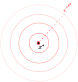
\includegraphics[width = 0.3\columnwidth]{../images/presentation/colapso.pdf}
	\end{center}
	\caption{\label{fig:colapso} Figura explicativa do surgimento da Bifurcação de Hopf.}
\end{figure}

\normalsize
\end{frame}%}}}2

%-----------------------------------------------------------------------------------------------------------------------
\begin{frame}%{{{2
\frametitle{Condições para a bifurcação de Hopf}
\scriptsize

	Da definição inferem-se duas condições para a bifurcação. A primeira, que um par de autovalores seja imaginário puro. A segunda, chamada \textit{Condição de transversalidade}, que os autovalores devem de fato transitar entre os semiplanos, quer dizer, não devem ``bater e voltar'' ou manter-se imaginários puros ao longo de uma faixa \cite{phdHopf}:

\begin{equation}
	\left. \dfrac{\partial \text{Re}\hspace{-0.5mm} \left(\lambda \right)}{\partial \mu} \right|_{\mu = \mu_B} \neq 0
\end{equation}

\normalsize
\end{frame}%}}}2

	
%-----------------------------------------------------------------------------------------------------------------------
\begin{frame}%{{{2
\frametitle{Lugar de raízes do sistema com AVR}
\scriptsize

\begin{figure}[htb]
	\begin{center}
	    \includegraphics[width = 0.9\columnwidth]{../images/presentation/lugarDeRaizesGeral.pdf}
	\end{center}
	\caption{\label{fig::lugarDeRaizes} Lugar de raízes do sistema controlado por AVR no equilíbrio $\vec{S} = 1 + j0.5$. A figura mostra o deslocamento de um autovalor do sistema em função dos parâmetros do controlador. Note-se que há também um autovalor conjugado ao ilustrado, que foi suprimido para melhor visualização.}
\end{figure}

\normalsize
\end{frame}%}}}2

%-----------------------------------------------------------------------------------------------------------------------
\begin{frame}%{{{2
\frametitle{Existência de bifurcação no sistema com AVR}
\scriptsize

	Na figura de lugar de raízes do sistema, pode-se notar que à medida que o ganho aumenta, os autovalores do sistema transitam do semiplano esquerdo para o direito, de forma que a cada valor de $T_e$ corresponda um valor de $K_e$ para os quais o par de autovalores depictado é imaginário. Nesse ponto, ocorre uma bifurcação: o ponto de equilíbrio transita de estável a instável.
\begin{figure}[htb]
	\begin{center}
	    \includegraphics[width = 0.5\columnwidth]{../images/presentation/existenciaDeBifurcacao.pdf}
	\end{center}
	\caption{\label{fig::existenciaDeBifurcacao} Ilustração do fenômeno de bifurcação.}
\end{figure}
\normalsize
\end{frame}%}}}2

%-----------------------------------------------------------------------------------------------------------------------
\begin{frame}%{{{2
\frametitle{Análise de autovalores do sistema com AVR}
\scriptsize

	O jacobiano do sistema controlado apenas por AVR é dado por

\begin{gather}
J = \left(\begin{array}{cccc}
J_{1,1} & 0 & J_{1,3} & J_{1,4} \\
%
J_{2,1} & 0 & J_{2,3} & 0 \\
%
0 & 1 & 0 & 0\\
%
J_{4,1} & 0 & J_{4,3} & J_{4,4}
\end{array} \right)
\end{gather}

	Daonde os autovalores são calculados por

\begin{align}
&\lambda^4 - \left( J_{1,1} + J_{4,4} \right)\lambda^3 + \left( J_{1,1}J_{4,4} - J_{1,4}J_{4,1} - J_{2,3}\right)\lambda^2 + \left[\strut J_{2,3}\left( J_{1,1} + J_{4,4}\right) - J_{1,3}J_{2,1}\right]\lambda + \nonumber \\[5mm] & \hspace{3cm} + J_{4,4}\left( J_{1,3}J_{2,1} - J_{1,1}J_{2,3}\right)  + J_{1,4}\left( J_{2,3}J_{4,1} - J_{2,1}J_{4,3}\right)= 0  \label{eq::polinomioJacobianoAVR} 
\end{align}

\normalsize
\end{frame}%}}}2

%-----------------------------------------------------------------------------------------------------------------------
\begin{frame}%{{{2
\frametitle{Parâmetros para bifurcação}
\scriptsize

	Pode-se mostrar que na bifurcação o ganho do controlador é função do tempo $T_e$ e do estado de equilíbrio, i.e., $K_{eB} = \mathbf{f}\left(T_e,x_0\right)$ onde $x_0$ é o vetor de estados no equiíbrio considerado

\begin{align}
&  \mathbf{K_{eB}} = \left[ \dfrac{J_{1,3}}{J_{1,4}\left(J_{1,1}\mathbf{T_e} - 1\right)}\right] \dfrac{ \left( J_{1,3}J_{2,1} - J_{1,1}J_{2,3}\right)\mathbf{T_e^3} + J_{2,3}\mathbf{T_e^2} + J_{1,1}\mathbf{T_e} - 1}{\left( J_{1,1}K_{4,3} - J_{1,3}K_{4,1} \right)\mathbf{T_e} - K_{4,3}} \label{eq::relacaoKeTe}
\end{align}

	Onde

\begin{gather}
\left\{ \begin{array}{l}
J_{4,1} = - K_{4,1} \dfrac{K_e}{T_e} \nonumber \\[5mm]
%
J_{4,3} = - K_{4,3} \dfrac{K_e}{T_e} \nonumber \\[5mm]
%
J_{4,4} = -\dfrac{1}{T_e} \nonumber
\end{array} \right.
\end{gather}

\normalsize
\end{frame}%}}}2

 %-----------------------------------------------------------------------------------------------------------------------
\begin{frame}%{{{2
\frametitle{Parâmetros para bifurcação}
\scriptsize

	Para o sistema em estudo, no ponto de equilíbrio, plota-se o ganho de bifurcação $K_{eB}$ contra $T_e$

\begin{figure}[htb]
	\begin{center}
	    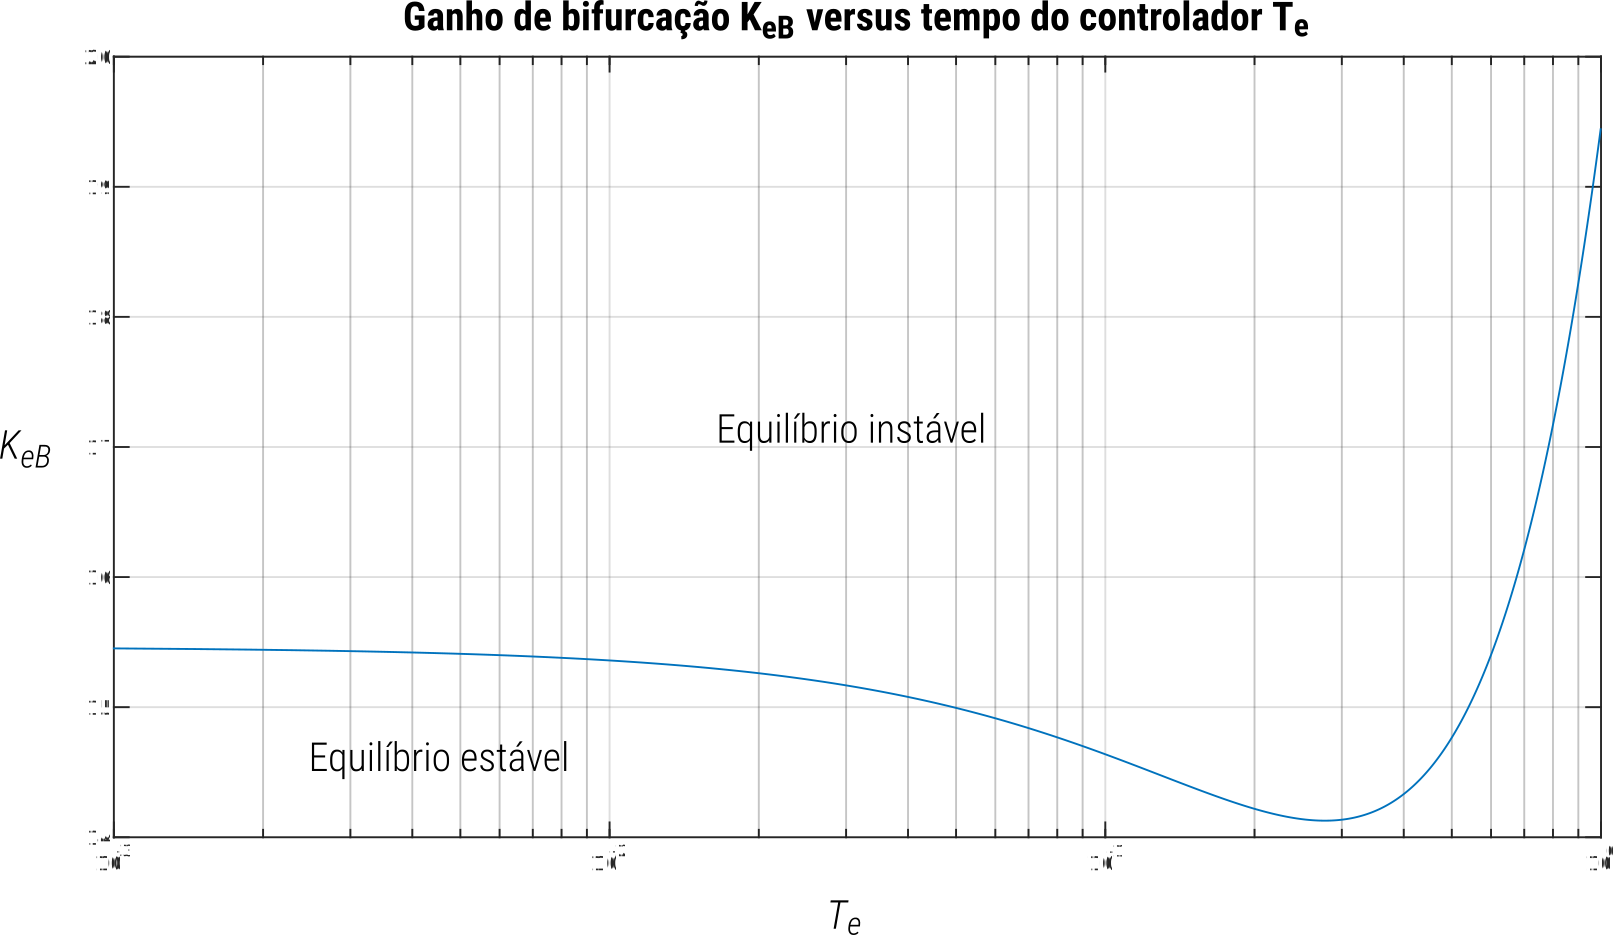
\includegraphics[width = 0.9\columnwidth]{../images/presentation/relacaoKeTe.pdf}
	\end{center}
	\caption{\label{fig::relacaoKeTe} Ganho de bifurcação $K_{eB}$ contra o tempo $T_e$ para o sistema em estudo.}
\end{figure}

\normalsize
\end{frame}%}}}2

%-----------------------------------------------------------------------------------------------------------------------
\begin{frame}%{{{2
\frametitle{Autovalores na bifurcação}
\scriptsize

	
	Em tempo, na bifurcação, os autovalores do sistema são
\begin{gather}
\left. \begin{array}{l}
a_3 = - \left( J_{1,1} + J_{4,4} \right) \\[5mm]
%
a_2 = \left( J_{1,1}J_{4,4} - J_{1,4}J_{4,1} - J_{2,3}\right) \\[5mm]
%
a_1 = \left[\strut J_{2,3}\left( J_{1,1} + J_{4,4}\right) - J_{1,3}J_{2,1}\right] \\[5mm]
%
a_0 = J_{4,4}\left( J_{1,3}J_{2,1} - J_{1,1}J_{2,3}\right) + \\[5mm] \hspace{4mm} + J_{1,4}\left( J_{2,3}J_{4,1} - J_{2,1}J_{4,3}\right)
\end{array} \right\}
%
\lambda = \left( \begin{array}{c}
-\dfrac{a_3}{2} + j\sqrt{\strut\ a_2 - \left(\dfrac{a_3}{2} \right)^2 - \dfrac{a_1}{a_3} } \\[5mm]
%
-\dfrac{a_3}{2} - j\sqrt{\strut\ a_2 - \left(\dfrac{a_3}{2} \right)^2 - \dfrac{a_1}{a_3} } \\[5mm]
%
+ j \sqrt{\strut \dfrac{\strut a_3}{a_1}} \\[5mm]
%
- j \sqrt{\strut \dfrac{\strut a_3}{a_1}}
\end{array} \right) \label{eq::autovaloresAVRBifurcacao}
\end{gather}

	Pode-se mostrar também que os dois primeiros autovalores são complexos Hurwitz-estáveis, uma vez que $a_3 > 0$.
\normalsize
\end{frame}%}}}2

%-----------------------------------------------------------------------------------------------------------------------
\section{Desenvolvimentos futuros} %{{{1
%-----------------------------------------------------------------------------------------------------------------------
\begin{frame}%{{{2
\frametitle{Desenvolvimentos futuros}
\small

\begin{itemize}
	\item Determinação das condições de bifurcação do sistema AVR+PSS;
%
	\item Cálculo dos tempos críticos de abertura dos sistemas. 
\end{itemize}

\normalsize
\end{frame}%}}}2

%%-----------------------------------------------------------------------------------------------------------------------
%\section{Agradecimentos}
%%-----------------------------------------------------------------------------------------------------------------------
%\begin{frame}%{{{2
%\frametitle{Agradecimentos}
%\scriptsize
%
%\begin{itemize}
%	\item Aos meus pais Álvaro Volpato Júnior e Eliane Bavaresco, pela educação e exemplos de índole; ao meu pai, especialmente, pelo exemplo de profissional e legado emocional que sempre vou carregar comigo;
%	%
%	\item À minha namorada Marina, pelo suporte infindável;
%	%
%	\item Ao orientador Luís Fernando Costa Alberto, pela paciência digna de um monge budista;
%	%
%	\item Aos professores Luís Fernando Costa Alberto, Rodrigo Andrade Ramos, Hildebrando Munhoz Rodrigues e Paulo Roberto Veronese, que me mostraram que inteligência não é um critério epistemológico -- mas sim ético.
%\end{itemize}
%
%\normalsize
%\end{frame}%}}}2
%
% \appendix
%-----------------------------------------------------------------------------------------------------------------------
\begin{frame}[allowframebreaks]%{{{2
\frametitle{Bibliografia}

\setbeamertemplate{bibliography item}[text]
\bibliographystyle{acm}
\nocite{*}
\bibliography{refs}

\end{frame}%}}}2
 
\end{document}
 
 
 
 


